% chktex-file 44
%%%%%%%%%%%%%%%%%%%%%%%%%%%%% Introduction %%%%%%%%%%%%%%%%%%%%

\chapter{Introduction}\label{cha:Introduction}

This thesis is concerned with the study of an X--ray binary star
system,\\%
% WHITE SPACE %
\groj, which is thought to harbour a black hole. Before
discussing this particular system in detail, a general introduction is
given to black holes and X--ray binaries. %

%%%%%%%%%%%%%%%%%%%%%%%%%%%%% Black Holes %%%%%%%%%%%%%%%%%%%%

\section{Black Holes}\label{cha:Introduction:sec:BlackHoles}

Possibly the most spectacular event in astrophysics is the death of a
``massive'' star, which is a star of mass greater than eight solar
masses. After millions of years of phenomenal energy output, the star
finally runs out of fuel. Most massive stars are then thought to form
dense cores, called \textbf{compact objects}, and some eventually
destroy themselves almost entirely. Such stars become a type of
compact objects called \textbf{black holes}. This section introduces
this exotic type of star and we will later explain the search for
evidence of the existence of black holes. %

\vspace{\myparskip}

Once a massive particle feels the gravitational attraction of a mass $M$, it
requires a certain velocity, called the \textbf{escape velocity
($v_{esc}$)}, to remove itself from that gravitational attraction. This
velocity is given by the formula:
\begin{equation} \label{cha:Introduction:sec:BlackHoles:eqn:V_Esc}
v_{esc} = \sqrt{\frac{2 G M}{r}},
\end{equation}
where $r$ is the distance between the masses, and $G$ is the
Gravitational constant. At the end of the 18th Century, Michell and Laplace suggested the
possibility of massive stars with $v_{esc} > c$. (Here, $c$ is the
speed of light in a vacuum.) These objects would always appear as
black stars. With the development of Einstein's General Theory of
Relativity, the modern picture of these ``black holes'' evolved: it is
now thought that a black hole remnant is formed when a star of
mass greater than ten solar masses ends its life cycle with a direct gravitational collapse. %
The matter remaining in the core of the star is totally devoid of
nuclear fuel and hence is compressed by gravity until it converges to a singularity - a black hole. %

%%%%%%%%%%%%%%%%%%%%%%%%%%%%% The Event Horizon %%%%%%%%%%%%%%%%%%%%

\subsubsection{The Schwarzschild Radius: the Size of the Black Hole}\label{cha:Introduction:sec:BlackHoles:subsubsec:EventHorizon}

It is thought that each black hole is surrounded by an \textbf{event
horizon}. This imaginary surface signifies the point of no return for any particle of mass
or radiation: once the particle has passed beyond the event horizon,
it is forever bound to the black hole. Not even light can escape, once it crosses this surface. Hence the compact object appears ``black''. %

\vspace{\myparskip}

All the points on the event horizon are a certain distance from the black hole, called the
\textbf{Schwarzschild radius ($R_{Sch}$)}. %
At this radius, which is given by:
\begin{equation}\label{cha:Introduction:sec:BlackHoles:eqn:R_Sch}
R_{Sch} = \frac{2 G M}{c^2},
\end{equation}
the escape velocity equals the speed of light. This radius is often used to characterise the size of the black hole -- these objects have no surface radius, being singularities. %

%%%%%%%%%%%%%%%%%%%%%%%%%%%%% How Can We Observe a Black Star in a Black Sky? %%%%%%%%%%%%%%%%%%%%

\subsubsection{How Can We Observe a Black Star in a Black Sky?}\label{cha:Introduction:sec:BlackHoles:subsubsec:HowCanWeObserveABlackStarInABlackSky}

It is difficult to observe isolated black holes directly, as they emit
very little radiation. However, the gravitational field caused by the mass of
the black hole is more easily detected, especially if the black hole
is gravitationally bound to a nearby star. When two stars are bound
together like this by their mutual gravitational attraction, the pair is known
as a \textbf{binary system}. We will later explore the specifics of
binaries containing black holes, but we first briefly summarize various topics
related to binary systems in general. %

%%%%%%%%%%%%%%%%%%%%%%%%%%%%% Binary Star Systems %%%%%%%%%%%%%%%%%%%%

\section{Binary Star Systems}\label{cha:Introduction:sec:BinaryStarSystems}

The majority of ``stars'' seen in the night sky are in fact multiple--star systems, each of which contain two or more mutually-bound stars. Here we examine the characteristics of binary star systems.

%%%%%%%%%%%%%%%%%%%%%%%%%%%%% Properties of a Binary System %%%%%%%%%%%%%%%%%%%%

\subsection{Properties of a Binary System}\label{cha:Introduction:sec:BinaryStarSystems:subsec:Properties}

The relative positions of the two component
stars in a binary system to the observer is known as the
\textbf{orbital phase}. Because the two stars in a binary system are orbiting about a common
centre of gravity, the appearance of the system to an observer changes as the stars rotate, and the orbital phase of the system changes. (Figure~%
\vref{cha:Introduction:sec:X--rayBinaries:fig:PringlePhaseEdited}%
\ shows various different phases for a type of binary system known as a
\textbf{Cataclysmic Variable}%
). At \textbf{phase 0.0}, the observer sees the \textbf{secondary}
(less massive) star in front of the \textbf{primary} star, and at
\textbf{phase 0.5}, the secondary is behind. The primary star and secondary star are observed side by
side at \textbf{phases 0.25} and \textbf{0.75}: these phases are known
as the \textbf{quadratures}. (Phases 0.0 and 0.5 are similarly known
as the \textbf{conjunctions}.) Note the time taken for the binary
system to rotate through one complete cycle of phases is known as the \textbf{orbital period ($P$)}. %

\vspace{\myparskip}

The appearance of a binary system also depends on other properties of
the system, such as:
\begin{itemize}
\item
the \textbf{mass of the primary}, $M_1$, and the \textbf{mass of the secondary}, $M_2$ -- the quantity $q = M_{1}/M_{2}$ is known as the \textbf{mass ratio}, %
\item
the \textbf{angle of orbital inclination}, $i$, which is the angle
between the observer and the normal to the orbital plane , and %
\item
the \textbf{binary separation}, which is the distance between the two stars. %
\end{itemize}

%%%%%%%%%%%%%%%%%%%%%%%%%%%%% Ellipsoidal Variability %%%%%%%%%%%%%%%%%%%%

\subsection{Ellipsoidal Variability of a Distorted Star}\label{cha:Introduction:sec:X--rayBinaries:subsec:EllipsoidalVariability}

When the binary separation of a system is roughly comparable to the
diameter of the star with the largest volume, the pair is called a
\textbf{close binary system}. %
The rotational and tidal forces acting on a star within a close binary
system can cause a stretching of the star into a tear-drop shaped
figure. In this thesis, most of the secondary stars in the systems we discuss are deformed in this way. %

\vspace{\myparskip}

This deformation of the secondary star can modulate the brightness of the binary system. %
The apparent flux of the secondary varies as a function of orbital phase, because this flux is
proportional to the projected surface area %
visible to the observer. As the binary system rotates, we see the projected surface area of the secondary star change (see, for example, Figure~%
\vref{cha:Introduction:sec:X--rayBinaries:fig:PringlePhaseEdited}%
). The amplitude of this variability depends primarily on the angle of inclination ($i$) and the mass ratio ($q$). It is largest for $i=90\degr$. %

\vspace{\myparskip}

For a given $i$, the projected surface area of the secondary star is
at its maximum value at the quadratures. The flux from the secondary is therefore at
its maximum value at phases 0.25 and 0.75. In a similar manner, the
flux is at its minimum values at the conjunctions, when the secondary is observed end-on and the
projected surface area is approximately circular. %

\vspace{\myparskip}

Under normal circumstances (e.g., the star is in hydrostatic
equilibrium), the local radiation flux on the surface of a star is
proportional to the local surface gravity. %
This gives rise to \textbf{gravitational darkening}. %
At \textbf{inferior conjunction} of the secondary (phase 0.0), the tidally-undisturbed side of the
secondary star faces the observer. All the points on the surface of
the star are equidistant from the centre of the star, and hence have the
same surface gravity and flux. %
However, at \textbf{superior conjunction} (phase 0.5), the star presents its distorted side, where the surface gravity is at its lowest, and hence the surface brightness
is also at its lowest value. This results in a deeper minimum in the light curve of the secondary star at phase 0.5 than at phase 0.0.

%%%%%%%%%%%%%%%%%%%%%%%%%%%%% OB97Figure6Edited2 %%%%%%%%%%%%%%%%%%%%
\begin{figure}[htb]
\begin{center}
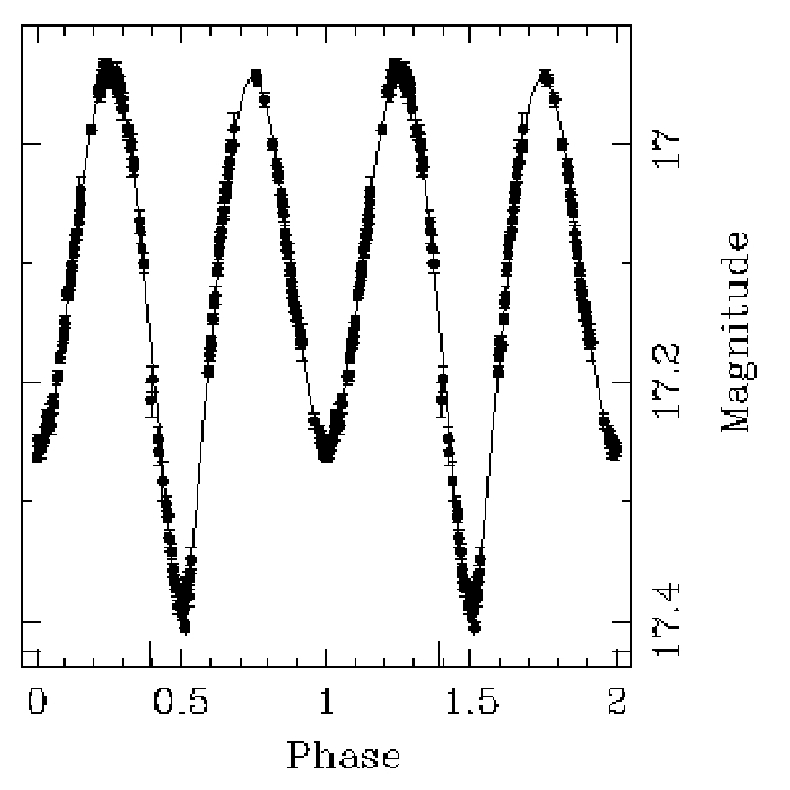
\includegraphics[width=9.2cm]{OB97Figure6Edited2}
\caption{%
Model fit to the optical light curve of the X--ray binary \groj,
showing the characteristic ellipsoidal variability of a distorted
secondary star. (Adapted from Orosz \& Bailyn 1997%
.)%
}\label{cha:Introduction:sec:X--rayBinaries:subsec:EllipsoidalVariability:fig:OB97Figure6Edited2}
\end{center}
\end{figure}
\nocite{OroszBailyn:1997} %
%%%%%%%%%%%%%%%%%%%%%%%%%%%%%%%%%%%%%%%%%%%%%%%%%%%%%%%%%%%%%%%%%%

\vspace{\myparskip}

In a binary system whose flux is dominated by that of the secondary
star, the light curve of the system will show the same ellipsoidal
variation as the secondary. An example of this \textbf{ellipsoidal
variability}, also known as \textbf{double hump modulation}, is given in Figure~%
\vref{cha:Introduction:sec:X--rayBinaries:subsec:EllipsoidalVariability:fig:OB97Figure6Edited2}%
. %

%%%%%%%%%%%%%%%%%%%%%%%%%%%%% Eclipses %%%%%%%%%%%%%%%%%%%%

\subsection{Eclipses in a Binary System}\label{cha:Introduction:sec:X--rayBinaries:subsec:Eclipses}

%%%%%%%%%%%%%%%%%%%%%%%%%%%%% WDEclipsing %%%%%%%%%%%%%%%%%%%%
\begin{figure}[!htb]
\begin{center}
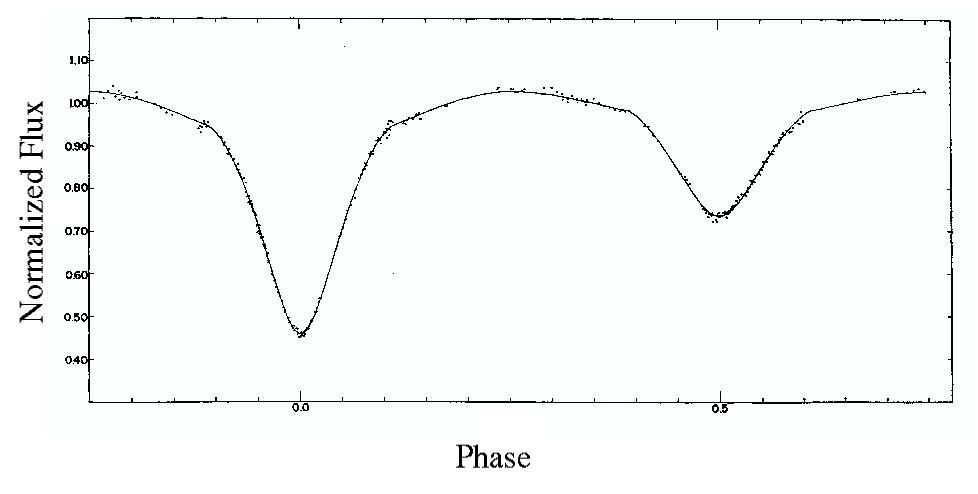
\includegraphics[width=15.0cm]{WDEclipsing}
\caption{%
Observations of the eclipsing binary WR Cyg, overplotted with a theoretical light curve. %
(Adapted from Wilson \& Devinney~1971.)%
}\label{cha:Introduction:sec:X--rayBinaries:subsec:Eclipses:fig:WDEclipsing}
\end{center}
\end{figure}
\nocite{WilsonDevinney:1971} %
%%%%%%%%%%%%%%%%%%%%%%%%%%%%%%%%%%%%%%%%%%%%%%%%%%%%%%%%%%%%%%%%%%



Another property of the light curve of a binary system is the presence
or absence of \textbf{eclipses}. When the orbital inclination of a binary system is high enough, the component stars in the system will travel in front of each other as they orbit the centre
of mass of the system. Since the closer star blocks the light of the
further, the total flux from the system diminishes. These \textbf{eclipses} may be the most prominent features of the light curve of the
binary. Of course, if the inclination is too low, no eclipses will
occur. Therefore, the presence or absence of eclipses puts a limit on
the value of the orbital inclination. Figure~%
\vref{cha:Introduction:sec:X--rayBinaries:subsec:Eclipses:fig:WDEclipsing}%
\ shows a model of an eclipsing system with the resultant light
curve. %

%%%%%%%%%%%%%%%%%%%%%%%%%%%%% Accretion %%%%%%%%%%%%%%%%%%%%

\subsection{Accretion onto the Primary}\label{cha:Introduction:sec:BinaryStarSystems:subsec:Accretion}

An important effect of the deformation of the secondary star in a close binary is the possible transfer of mass from one star to the other. This process is known as \textbf{accretion} or \textbf{mass transfer}. Whether it occurs depends on the sizes and separation of the component stars, as we now explain.%

%%%%%%%%%%%%%%%%%%%%%%%%%%%%% The Roche Lobes %%%%%%%%%%%%%%%%%%%%

\subsubsection{Accretion and the Roche Lobes}\label{cha:Introduction:sec:BinaryStarSystems:subsec:Accretion:subsubsec:RocheLobes}

During the 19th century, the French mathematician Edouard Roche
studied the interactions of planetary satellites. %
His work has been applied to binary systems to develop a theoretical
model for accretion.

%%%%%%%%%%%%%%%%%%%%%%%%%%%%% PringleRoche %%%%%%%%%%%%%%%%%%%%
\begin{figure}[!htb]
\begin{center}
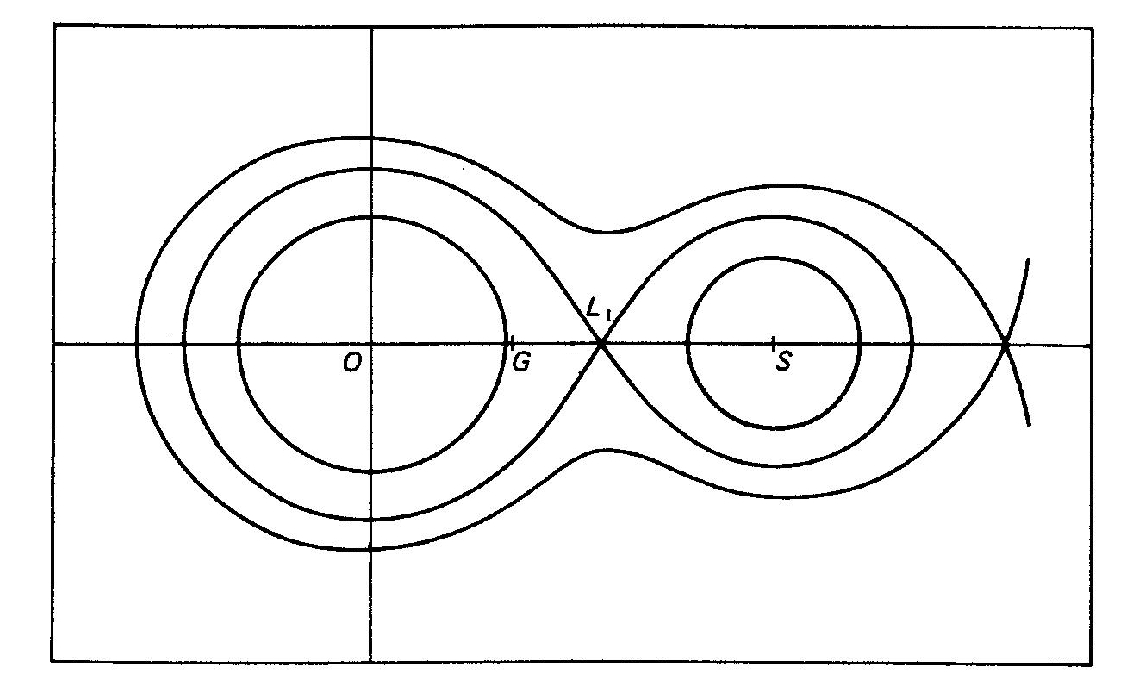
\includegraphics[width=10.0cm]{PringleRoche}
\caption{%
Example of the Roche equipotentials for a binary system.  The centre,
$O$, of the primary star is marked, as is
the centre, $S$, of the secondary star.  Also marked are
the Lagrangian point, $L_1$, and the centre of mass, $G$, of the
system. The mass ratio is given as $q = 2$. %
(Adapted from Pringle~1985.)%
}\label{cha:Introduction:sec:BinaryStarSystems:subsec:Accretion:subsubsec:RocheLobes:fig:PringleRoche}
\end{center}
\end{figure}
\nocite{Pringle:1985} %
%%%%%%%%%%%%%%%%%%%%%%%%%%%%%%%%%%%%%%%%%%%%%%%%%%%%%%%%%%%%%%%%%%

\vspace{\myparskip}

By studying the gravitational interaction between two objects, Roche
developed a series of curves representing equipotential surfaces
surrounding the pair (see Figure~%
\vref{cha:Introduction:sec:BinaryStarSystems:subsec:Accretion:subsubsec:RocheLobes:fig:PringleRoche}). The shape and size of these curves are determined by the mass ratio of
the two objects and their separation.  The most important curves are
the two so-called \textbf{Roche lobes}, the ``figure of 8'' shaped surface. %

\vspace{\myparskip}

As the \textbf{companion} (secondary) star evolves, %
its size increases and it may expand to fill its Roche lobe. Some of
the matter of that star may lie on or even outside this lobe, and some of this matter will
be attracted towards the primary. The gas will flow towards the
primary through the \textbf{inner Lagrangian point ($L_1$)}, %
which is the intersection of the Roche lobes. This process is known as
\textbf{Roche lobe overflow accretion}. %
Such a binary system is known as a \textbf{semi-detached binary}, if the radius of the primary star is less than its Roche lobe
radius. If the companion star of a binary system does not fill its
Roche lobe, then the stellar matter is bound and no mass transfer to
the primary occurs by Roche lobe accretion. In some such systems, mass
transfer can still occur via a
\textbf{stellar wind}, a stream of gas particles flowing out from the star, similar to the
solar wind. In this thesis, however, we are mainly concerned with
Roche lobe overflow accretion. %

\vspace{\myparskip}

The characteristics of binary systems that we have outlined are common to all binaries -- we now detail the specifics of the type of binary systems known as X--ray binaries. %

%%%%%%%%%%%%%%%%%%%%%%%%%%%%% X--ray Binaries %%%%%%%%%%%%%%%%%%%%

\section{X--ray Binaries}\label{cha:Introduction:sec:X--rayBinaries}

%%%%%%%%%%%%%%%%%%%%%%%%%%%%% PringlePhaseEdited %%%%%%%%%%%%%%%%%%%%
\begin{figure}[htb]
\begin{center}
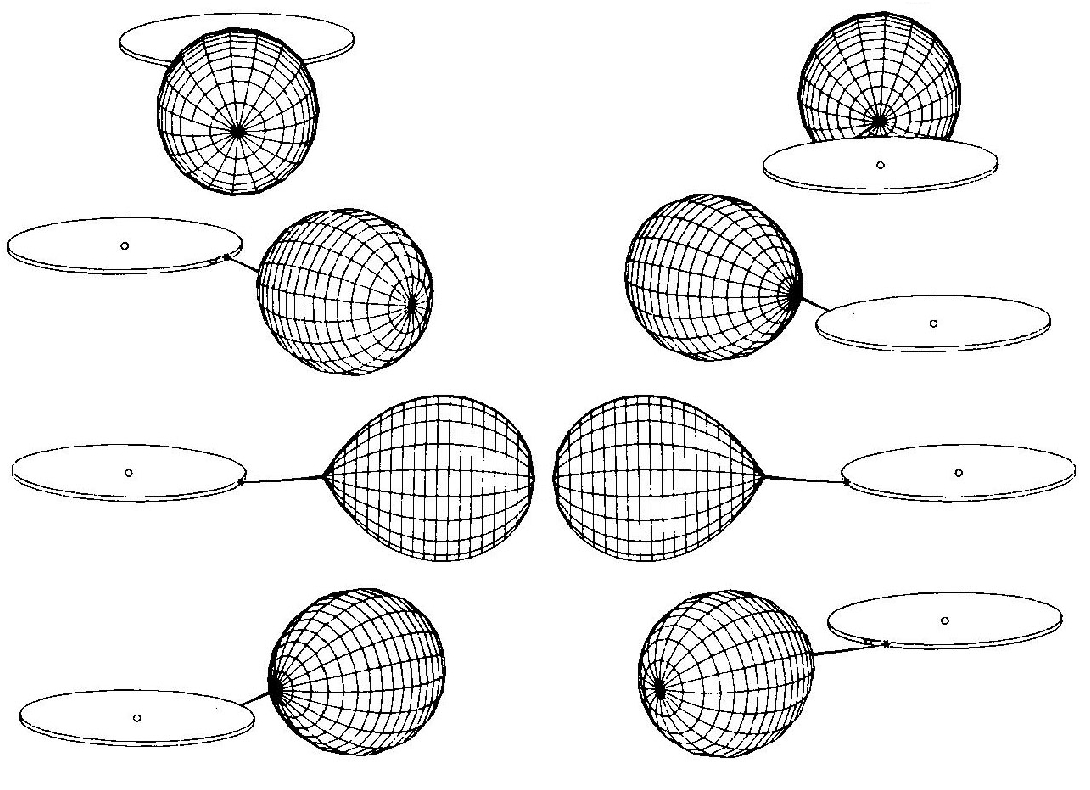
\includegraphics[width=10.0cm]{PringlePhaseEdited}
\caption{%
The observed relative positions of the component stars of a cataclysmic variable
as a function of orbital phase, beginning with phase 0.0. The
phase difference between images, going from top to bottom, is
0.125. (Adapted from %
Pringle \& Wade 1985.)%
}\label{cha:Introduction:sec:X--rayBinaries:fig:PringlePhaseEdited}
\end{center}
\end{figure}
\nocite{PringleWade:1985} %
%%%%%%%%%%%%%%%%%%%%%%%%%%%%%%%%%%%%%%%%%%%%%%%%%%%%%%%%%%%%%%%%%%

Many semi-detached binary systems have a compact primary star and a
non-degenerate secondary. (For the remainder of this discussion, such a
binary system will be assumed unless otherwise stated.) This compact
object may be a white dwarf, neutron star or black hole.

\vspace{\myparskip}

When the primary star of such a system is an accreting white dwarf, the system is a \textbf{cataclysmic variable} (see Figure~\vref{cha:Introduction:sec:X--rayBinaries:fig:PringlePhaseEdited} for an example): these variables are divided into such categories as the brighter \textbf{classical
  novae}, the fainter \textbf{dwarf novae}\label{cha:Introduction:sec:X--rayBinaries:subsec:CompactObjects:topic:DwarfNovae}%
 and the \textbf{novalike objects}. %
The radiation emitted by these systems is chiefly in the optical and ultraviolet regions
of the electromagnetic spectrum. %

When the primary in a close binary system is a neutron star or
black hole, the binary is called an \textbf{X--ray binary}.
X--ray binaries take their name from the fact that the majority of
the energy radiated from the bright systems during phases of high accretion is in the form of X--rays (with
energies 0.1--100\,keV). (We denote the mass of this X--ray emitting object by $M_{X}$.) In an X--ray binary, the radius of the compact primary will always be
less than its Roche lobe radius, hence these systems are
always semi-detached.


\vspace{\myparskip}

In 1962, Giacconi et~al.\ discovered the first known X--ray emitting cosmic
object in the constellation of Scorpius (Giacconi et~al.\ %
\citeyearNP{Giacconi_et_al.:1962}). %
The source, christened Sco X--1, was later shown to be a binary
system, and is usually the brightest X--ray binary in the sky. The
first confirmed X--ray binary, however, was \mbox{Cyg X--1} %
\cite{WebsterMurdin:1972,Bolton:1972}. %
Since this observation, approximately 300 X--ray binaries have been
identified %
(\citeNP{LiuVanParadijsVanDenHeuvel:2000},
\citeNP{LiuVanParadijsVanDenHeuvel:2001}).%

\vspace{\myparskip}

Once the first X--ray binaries had been identified optically, their
distances and hence their intrinsic X--ray luminosities were determined. Some of the luminosities calculated were of the order of $10^{31}\,\mathrm{W}$, which is approximately
$10^5\,\mathrm{L}\sun$ (where $\mathrm{L}\sun$ is the
luminosity of the Sun%
\footnote{\label{cha:Introduction:sec:X--rayBinaries:foot:Lsun}
$1\,\mathrm{L}\sun = 3.826 \times 10^{26}\,\mathrm{W}$ }%
).\label{cha:Introduction:sec:X--rayBinaries:subsec:CompactObjects:topic:HighLum}
\citeN{Shklovsky:1967:ApJL} %
suggested that this unusually high luminosity of X--ray binaries such as
Sco X--1 could be accounted for if they were mass-exchanging binaries
with a neutron star component. %
This was the first realisation that accretion was an important power
source. Much of the energy radiated by these systems comes from a disk of gas around the primary star -- the \textbf{accretion disk}.

%%%%%%%%%%%%%%%%%%%%%%%%%%%%% Accretion Disk %%%%%%%%%%%%%%%%%%%%

\subsection{The Accretion Disk}\label{cha:Introduction:sec:BinaryStarSystems:subsec:AccretionDisk}

In a binary where accretion is taking place, if there is a continual stream of particles flowing from the
the secondary star to the primary, the gas forms a disk, known as the
\textbf{accretion disk}. %
The rotation of the secondary star imparts angular momentum to the matter flowing into this disk.
Viscous processes redistribute the angular momentum amongst the
gas particles, which causes the in--falling of some of the particles onto the primary. The in--falling
gas is heated until it forms a highly ionized plasma, with highest
temperatures closest to the primary. %

\vspace{\myparskip}

An accretion disk is very efficient at converting the gravitational potential energy of the transferred matter into radiation. For example, about 20\% (for a neutron star primary) or 30\% (for a
black hole primary) of the rest energy of the accreted gas may be
emitted as radiation. The accretion results in a luminosity of the primary given by:
\begin{equation} \label{cha:Introduction:sec:X--rayBinaries:subsec:AccretionDisk:eqn:LumAcc}
L = \frac{G M_X \dot{m}}{R_X},
\end{equation}
where $R_X$ is the radius of the primary star, and $\dot{m}$ is the
rate of mass transfer from the secondary star onto the primary star. %
(Note that this formula does not strictly apply to black holes, as it assume a
primary star with a hard surface.) %
There exists an upper limit for $L$, called the \textbf{Eddington
Limit ($L_{E}$)}\label{cha:Introduction:sec:BinaryStarSystems:subsec:AccretionDisk:topic:L_E}%
, above which the outer parts of the star cannot remain in hydrostatic
equilibrium. Above $L_{E}$, the process of accretion is halted due to
the radiative pressure from the star, and in fact mass loss from the primary may occur. %

\vspace{\myparskip}

Using Equation~%
\vref{cha:Introduction:sec:X--rayBinaries:subsec:AccretionDisk:eqn:LumAcc}, %
and assuming a solar mass primary, we see
that the high luminosities mentioned on page~%
\pageref{cha:Introduction:sec:X--rayBinaries:subsec:CompactObjects:topic:HighLum}%
\ can be generated by an accretion rate of
only $10^{-8}\,\mathrm{M}\sun\,\mathrm{yr^{-1}}$ (e.g., %
\citeNP{Fabian:1985}%
), %
reflecting the aforementioned efficiency of accretion as a power
source. (Here $\mathrm{M}\sun$\ is the mass of the Sun%
\footnote{\label{cha:Introduction:sec:X--rayBinaries:foot:Msun}
$1\,\mathrm{M}\sun = 1.99 \times 10^{30}\,\mathrm{kg}$}%
.)

%%%%%%%%%%%%%%%%%%%%%%%%%%%%% Reprocessing of Radiation %%%%%%%%%%%%%%%%%%%%

\subsubsection{Reprocessing of Radiation}\label{cha:Introduction:sec:X--rayBinaries:subsec:AccretionDisk:subsubsec:ReprocessingOfRadiation}

An important effect of accretion in the case of X--ray binaries is a
process called \textbf{X--ray reprocessing} or \textbf{X--ray heating}. The X--ray radiation emitted by the
accreting material interacts with the matter in the accretion disk, in
the secondary star or surrounding the binary system. This interaction
converts some of the emission into optical and infrared (IR) radiation. This
X--ray heating can affect the appearance of the disk and the secondary
star, as we will later see. %

%%%%%%%%%%%%%%%%%%%%%%%%%%%%% Categorization of X--ray Binaries %%%%%%%%%%%%%%%%%%%%

\subsection{Categorisation of X--ray Binaries}\label{cha:Introduction:sec:X--rayBinaries:subsec:CategorizationOfX--rayBinaries}

X--ray binaries are generally categorized by the mass of the
secondary star, which is classified as either a high mass or a low
mass star. The two corresponding categories are the \textbf{High-Mass
X--ray Binaries (HMXBs)} and the \textbf{Low-Mass X--ray Binaries (LMXBs)}. %
As well as mass distinctions, X--ray binary systems can be divided into
two categories on the basis of the variability of their luminosity: %
X--ray binaries which display transient high-energy emissions are known as
\textbf{transient X--ray binaries}, while those with persistently bright behaviour are known as
\textbf{persistent X--ray binaries}. We first consider the two mass--related categories. %

%%%%%%%%%%%%%%%%%%%%%%%%%%%%% High-Mass X--ray Binaries %%%%%%%%%%%%%%%%%%%%

\subsection{High-Mass X--ray Binaries (HMXBs)}\label{cha:Introduction:sec:X--rayBinaries:subsec:HMXBs}

High-Mass X--ray Binaries contain companion stars with masses of $\gsim$
10\,M\sun. These stars are O or B giants or supergiants, %
with temperatures of roughly 20,000\,K, %
and have survived the supernova explosion of their evolved
companion. %
The compact object in the majority of HMXBs (67 of the 70 known) is a pulsating neutron
star.
The other three HMXBs are thought to harbour black holes, and are persistent sources. %

\vspace{\myparskip}

HMXBs tend to have large binary separations (due to the giant size of
the secondary) and therefore long orbital periods. The periods range from 4.8 hours to 188 days
\cite{VanParadijs:1995}, with the eccentricity of the orbit increasing with the period. %

\vspace{\myparskip}

Despite this large separation, the size of the secondary star may
permit mass transfer onto the primary via a stellar wind or even Roche lobe
overflow accretion. %
Mass loss rates of between $10^{-6}$ and $10^{-10}$\,M\sun $\mathrm{yr}^{-1}$ can be
achieved by stellar winds %
\cite{WhiteNagaseParmar:1995}, %
and the compact object captures a small fraction of this mass. %

\vspace{\myparskip}

One of the main characteristic of a typical HMXB is the observation of
\textbf{outbursts}, or high brightness states, at regular intervals,
caused by the interaction of the neutron star with the stellar wind
surrounding the
secondary star. The companion dominates the optical and infrared
luminosity of the system, but X--ray reprocessing and the presence of an accretion disk do modulate
this luminosity. %

%%%%%%%%%%%%%%%%%%%%%%%%%%%%% Low-Mass X--ray Binaries %%%%%%%%%%%%%%%%%%%%

\subsection{Low-Mass X--ray Binaries (LMXBs)}\label{cha:Introduction:sec:X--rayBinaries:subsec:LMXBs}

The secondary star of an LMXB has a mass of $\lsim 1\,\mathrm{M}\sun$
and is generally a K or M dwarf star. The number of observed LMXBs is greater than that of observed HMXBs: %
\citeN{TanakaLewin:1995} %
estimate the number of known LMXBs to be about 125, with 39 observed
X--ray transient LMXBs. Of these 125, 17 LMXBs are thought to contain black holes, with 14 in X--ray transient systems. %

\vspace{\myparskip}

The size of the companion star determines the binary separation, as a
small companion requires a small separation in order for mass transfer to
occur. The orbital period of the binary system is therefore affected by the
nature of the companion. Systems with dwarf companions have
periods of the order of hours, whereas binaries containing evolved
companion stars have orbital periods of the order of days. The periods of known LMXBs range from 11.4 minutes to 16.6 days %
\cite{VanParadijs:1995}. %
The shortest periods are possible only because of the low mass of the
companion star. %

\vspace{\myparskip}

The category of Low Mass X--ray Binaries can be divided into two
sub-categories:

\begin{itemize}
\item %
The systems which are continually bright are denoted
\textbf{persistent LMXBs}, and almost all of these contain neutron stars. %
The accretion disk is brighter than the secondary star for almost all of the persistent
LMXBs. Therefore the optical spectrum is that of the hot disk with emission lines superimposed (see, e.g., Shahbaz et~al.\ %
\citeyearNP{Shahbaz_et_al.:1996}%
) and appears blue. The spectrum of the secondary star is only
observable for those persistent LMXBs with long orbital periods. %

\item %
The LMXBs which exhibit transient behaviour are known as \textbf{soft
X--ray transients (SXTs)}. Most SXTs ($\geq 70\%$) are thought to contain black holes.
One reason these transients are studied is that it is possible to observe the secondary star during the long periods of quiescence. Another benefit is that the large range in
luminosities of these objects allows accretion models to be tested
over a range of mass accretion rates for a given system. Neither of these are possible with the persistently bright sources. %


\end{itemize}
It is to these transient LMXBs that we now direct our attention. %


%%%%%%%%%%%%%%%%%%%%%%%%%%%%% Soft X--ray Transients %%%%%%%%%%%%%%%%%%%%

\subsection{Soft X--ray Transients (SXTs)}\label{cha:Introduction:sec:X--rayBinaries:subsec:SXTs}

Harries et al.\ %
\citeyear{Harries_et_al.:1967} %
discovered the first \textbf{Soft X--ray Transient}, %
Cen X--2, when they detected a very bright X--ray source %
during rocket flights. %
At its peak, this bright source outshone Sco X--1, but it later
diminished. Transients like Cen X--2 were first studied in the 2--10\,keV range, where a
soft component in their spectra can be seen. This led to their
designation as soft X--ray transients, even though they often exhibit
very hard spectra at higher energies. %

\vspace{\myparskip}

All soft X--ray transients display the two state behaviour of Cen X--2. The low
accretion and low brightness state, or
\textbf{quiescence}, can last for months to decades. The \textbf{outburst}
state occurs when the accretion rate onto the
compact object is dramatically increased (in some cases caused most
likely by an instability in the accretion disk), with a corresponding increase in luminosity.
These outbursts last only briefly, but the outbursts of many, if not all, transients are recurrent.
 The luminosity of a soft X--ray transient typically increases by a factor
of $10^3$--$10^4$ as the system passes from its quiescent phase into
outburst, and the outburst luminosity is usually between
$10^{30}\,\mathrm{W}$ and $10^{32}\,\mathrm{W}$ %
\cite{TanakaLewin:1995}. %

\vspace{\myparskip}

Since the discovery of Cen X-2, approximately 23 SXTs have been
observed, of which only 25\% contain neutron stars. SXTs are now being
discovered at a rate of 1 or 2 per year. The prototype SXT is A0620-00
(\mbox{Nova Mon 1975}), noted by Elvis et~al.\ %
\citeyear{Elvis_et_al.:1975}%
\ to be the brightest extrasolar X--ray source for several months. %
Indeed, when in outburst, SXTs are among the brightest sources in the X--ray, but they may be undetectable in this region of the spectrum during quiescence. %

\vspace{\myparskip}

Because of the large change in the brightness of SXTs from quiescence
to outburst, and because both SXTs and dwarf novae (see page~%
\pageref{cha:Introduction:sec:X--rayBinaries:subsec:CompactObjects:topic:DwarfNovae}%
) have variable accretion rates, SXTs are also known by the less accurate term \textbf{X--ray novae
(XRNe)}. The disk instability models applied to dwarf novae have been adapted for
SXTs (see, e.g., %
\citeNP{Meyer-HofmeisterMeyer:2000}%
), but the effect of the X--ray irradiation of the disk and the secondary must
also be taken into account. Nevertheless, these models should hold for SXTs during quiescence,
where there is negligible X--ray heating of the secondary and the
disk. %

\vspace{\myparskip}

%%%%%%%%%%%%%%%%%%%%%%%%%%%%% Classifying an LMXB as Transient %%%%%%%%%%%%%%%%%%%%

Because all LMXBs vary to some extent, some criteria must be applied to determine whether a LMXB is a persistent or transient source. An LMXB is generally denoted as an SXT if the following holds %
\cite{TanakaShibazaki:1996}:
\begin{enumerate}
\item\label{cha:Introduction:sec:X--rayBinaries:subsec:CriteriaForSXTs:enu:flux}
The X--ray flux from the binary has rapidly increased from its quiescent
value by more than two orders of magnitude within only a few days.
\item\label{cha:Introduction:sec:X--rayBinaries:subsec:CriteriaForSXTs:enu:reduction}
The flux has then been reduced (exponentially) to its quiescent value
over a period of about 10--100 days.
\item\label{cha:Introduction:sec:X--rayBinaries:subsec:CriteriaForSXTs:enu:outburst}
If the outburst has recurred, the time scale of the outburst was
smaller than the quiescent stage (typically decades: Hynes et~al.\ %
\citeyearNP{Hynes_et_al.:1998}). %
\item\label{cha:Introduction:sec:X--rayBinaries:subsec:CriteriaForSXTs:enu:recur}
The outburst has not recurred with a regular period.
\end{enumerate}

%%%%%%%%%%%%%%%%%%%%%%%%%%%%% Outburst %%%%%%%%%%%%%%%%%%%%

\subsection{SXTs in Outburst}\label{cha:Introduction:sec:X--rayBinaries:subsec:Outburst}

During X--ray outburst, the X--ray luminosity, $L_X$, of an SXT increases until it reaches
the Eddington limit (see%
\ \vref{cha:Introduction:sec:BinaryStarSystems:subsec:AccretionDisk:topic:L_E}%
). Outbursts at optical wavelengths are also observed.%

\vspace{\myparskip}

In many SXTs the solid angle of the secondary, viewed from the compact star, is small, and so the reprocessing
of X--rays takes place mainly in the accretion disk, rather than the secondary. A typical accretion disk in a transient LMXB during outburst is illuminated by approximately one quarter of the
flux from the compact star, or approximately
$10^{30}\,\mathrm{W}$ %
\cite{VanParadijsMcClintock:1995}. %
The resultant intense heating of the disk causes the luminosity of the
disk to be far greater than that of the faint K or M dwarf secondary,
which is typically $10^{26}\,\mathrm{W}$. %
The change in the optical brightness of the SXT is therefore due to the changing
visibility of the accretion disk. The light curve has one maximum and minimum per orbital
cycle, and the minimum occurs when the secondary is closest to the
observer. %

\vspace{\myparskip}

This dominance of the disk contribution to the optical brightness means
that ellipsoidal variations are only observed during the quiescent
states of transient LMXBs. During
quiescence, the X--rays are mostly absent and the disk and secondary are not
significantly heated. %

%%%%%%%%%%%%%%%%%%%%%%%%%%%%% Quiescence %%%%%%%%%%%%%%%%%%%%

\subsection{The Quiescent Period of an SXT}\label{cha:Introduction:sec:X--rayBinaries:subsec:Quiescence}

During quiescence, the weak emissions from the dwarf secondary should dominate the optical and
infrared. Hence, the ellipsoidal variability due to the secondary is
observable directly during this state. %

\vspace{\myparskip}

The disk is hotter than the secondary, however, and therefore it contributes more at shorter wavelengths.
The disk also contributes a constant flux offset and
possible random flickering. This aperiodic flickering may cause the light curve to change
from one observation to the next (see, e.g., Chevalier et~al.\ %
\citeyearNP{Chevalier_et_al.:1989})%
, and the veiling of the secondary by the accretion disk reduces the
fractional amplitude of the ellipsoidal variability. %

\vspace{\myparskip}

During quiescence, mass transfer continues, suggesting the Roche lobe
of the secondary remains filled. The quiescent X--ray luminosity,
$L_X$, is of the order of $10^{23}$--$10^{26}\,\mathrm{W}$, and is
usually much less than the optical luminosity.

%%%%%%%%%%%%%%%%%%%%%%%%%%%%% Black Hole Candidates within Soft X--ray Transients %%%%%%%%%%%%%%%%%%%%

\subsection{SXTs and Black Holes}\label{cha:Introduction:sec:X--rayBinaries:subsec:BHCSXTs}

Soft X--ray transients have proved very important in the study of
black holes. It is difficult to distinguish between an X--ray binary containing a neutron star and one harbouring a black hole. One possible criterion for differentiating between neutron stars and
black holes is the mass of the star: \citeN{RhoadesRuffini:1974}%
\ and %
\citeN{ChitreHartle:1976} %
showed that the maximum mass of a neutron star is approximately
$3\,\mathrm{M}\sun$. %
This limit is based on certain assumptions, such as that General Relativity
is the correct theory of gravity, and that causality holds inside the
neutron star (i.e., sound cannot travel faster than light). Nevertheless, compact objects with masses greater than this limit are generally considered to be black holes.

\vspace{\myparskip}

\begin{table}[htb]
\caption{Two of the Best Studied SXTs with BHC Primaries}\label{cha:Introduction:sec:X--rayBinaries:subsec:BHCSXTs:tab:SummaryOfObservationsSXTBHC}

\begin{minipage}{\linewidth}
\renewcommand{\thefootnote}{\thempfootnote}

\DeclareFixedFootnote{\period}{The orbital period of the binary.} % For fixed footnote

\begin{center}
\begin{tabular}{|l||||c|c|c|}

\hline
System & $f(M_X)$/M\sun  & $M_X$/M\sun & $P\period$ \\\hline\hline\hline\hline
V404 Cyg\footnote{\citeN{CasaresCharlesNaylor:1992}} & $6.26\pm0.31$ & 8--12 & $6\fd473\pm0\fd001$
\\\hline
A0620-00\footnote{\citeN{McClintockRemillard:1986}} & $3.18\pm0.16$ & 7--15 & $7\fh75234\pm0\fh0010$
\\\hline
%\groj\ & $2.73\pm0.09$\footnote{\citeN{Shahbaz_et_al.:1999}} &
%$5.4\pm0.3$\footnote{\citeN{BeerPodsiadlowski:2001}} &
%$2\fd62168\pm0\fd00014$\footnote{van der Hooft et~al.\ %citeyear{VanDerHooft_et_al.:1998}}\\\hline
\hline
\end{tabular}
\end{center}
\end{minipage}
\end{table}

\citeN{WebsterMurdin:1972} %
and %
\citeN{Bolton:1972} %
discovered the first BHC in the binary system Cyg X-1, which has a
primary with a mass of $\gsim 3$\,M\sun. Since then, the increase in the number of strong Galactic BHCs is in part due to
the discovery of SXTs: a remarkably high fraction%
\footnote{\label{cha:Introduction:sec:X--rayBinaries:subsec:BHCSXTs:foot:fraction}%
A higher fraction than any other class of Galactic X--ray sources.%
}%
\ of the SXTs currently known are thought to
harbour black holes%
\ \cite{VanParadijs:1998}%
. Table~%
\vref{cha:Introduction:sec:X--rayBinaries:subsec:BHCSXTs:tab:SummaryOfObservationsSXTBHC}%
\ lists two of the best known soft X--ray transients containing black hole candidates, together with their system properties. %

\vspace{\myparskip}

The detection of a high fraction of SXTs containing BHCs is due to the lower accretion rates for systems with black holes, and to the extended periods of quiescence in
SXTs, as we now explain:
\begin{itemize}

\item
The accretion rate for an X--ray binary generally decreases as the mass
of the primary increases and the secondary star evolves %
\cite{Casares:2001}%
. Therefore, binaries with the more massive black holes are more
likely to be transient sources than those with neutron stars, as their
accretion rates are more likely to be below the critical accretion
rate%
\footnote{\label{cha:Introduction:sec:X--rayBinaries:subsec:BHCSXTs:foot:CritAccRate}%
A system will be transient or persistent depending on its accretion rate. The \textbf{critical accretion rate} is the rate above which the system will be persistent. %
}%
\ \cite{KingKolbBurderi:1996}. This also accounts for why most SXTs have highly evolved
secondaries. %

\item
Also, the extended periods of quiescence, absent from persistent
sources, enable accurate determination of the component masses of the
binaries. It is therefore more likely that compelling evidence of a
black hole would be found in an SXT rather than in another persistently bright X--ray binary with
similar system properties. %

\end{itemize}

Many of the X--ray peculiarities of Cyg X--1, the first BHC, were
originally assumed to indicate the black hole nature of a
source %
\cite{TanakaLewin:1995}%
. These characteristics were :
\begin{enumerate}
\item\label{cha:Introduction:sec:X--rayBinaries:subsec:BHCSXTs:enu:ultrasoft}
an ultrasoft X--ray spectrum,
\item\label{cha:Introduction:sec:X--rayBinaries:subsec:BHCSXTs:enu:millisecond}
millisecond X--ray flickering,
\item\label{cha:Introduction:sec:X--rayBinaries:subsec:BHCSXTs:enu:twostates}
a high, soft state and a low hard X--ray state, and
\item\label{cha:Introduction:sec:X--rayBinaries:subsec:BHCSXTs:enu:hardtail}
a hard X--ray tail.
\end{enumerate}
However, neutron star systems, such as Cir X--1 and X0331+53, have also
been shown to display these properties. Although the presence of properties similar to these
characteristics of Cyg X--1 are indeed suggestive of a black hole
nature, the most persuasive determination is the calculation of the
mass of the collapsed star. A lower limit to this mass can be made by calculating the
\textbf{mass function} of the star. %

%%%%%%%%%%%%%%%%%%%%%%%%%%%%% The Mass Function %%%%%%%%%%%%%%%%%%%%

\subsection{The Mass Function}\label{cha:Introduction:sec:X--rayBinaries:subsec:MassFunction}

Applying Kepler's Laws to the binary system, it is possible to derive the following result:
\begin{equation}\label{cha:Introduction:sec:X--rayBinaries:subsec:MassFunction:eqn:MassFn}
\frac{M_X^3 \sin^3{i}}{(M_X+M_2)^2} = \frac{P K_2^3}{2 \pi G},
\end{equation}
where $K_2$ is the \textbf{radial velocity} semi-amplitude%
\footnote{\label{cha:Introduction:sec:X--rayBinaries:subsec:MassFunction:foot:radial}%
The \textbf{radial velocity} of a star is the velocity of the star along the line of sight of
the observer. The semi-amplitude of the radial velocity is normally
measured by calculating the Doppler shift of absorption features in
the spectrum of the secondary star. %
}%
\  of the secondary star.%
\ The right hand side of Equation~%
\ref{cha:Introduction:sec:X--rayBinaries:subsec:MassFunction:eqn:MassFn}%
\ is defined to be the \textbf{mass function of the primary star,
  $f(M_X)$}, and is a lower limit approximation of the mass of the
compact object, since the left hand side of this equation is always $\leq M_X$. A
similar definition can be made for the mass function of the companion $f(M_2)$,
which gives a lower limit for the mass of the companion. %

\vspace{\myparskip}

Since the mass function of the primary
star sets a lower limit for the mass of the star, finding a primary
whose mass function is above the limit of %
\citeN{RhoadesRuffini:1974}%
\ suggests that the star is a black hole. One of the
highest mass functions yet measured is that of \mbox{XTE J1555--564}
($6.86\pm0.71\,\mathrm{M}\sun$: Orosz et~al.\ %
\citeyearNP{Orosz_et_al.:2002}
), well above the neutron star limit. %

%%%%%%%%% Determining the Mass of the Primary %%%%%%%%%%%%%%%%%%%%

\subsection{Determining the Mass of the Primary}\label{cha:Introduction:sec:X--rayBinaries:subsec:DeterminingTheMassOfThePrimary}

Rather than setting a limit to the mass of the primary using the mass
function, if we can constrain the mass of the secondary (say from
consideration of its spectral type), we can calculate $M_{X}$ from the
mass ratio $q$. But first we must constrain $q$ and $i$. %

\vspace{\myparskip}

The simplest method to calculate $q$ is to determine the velocity
curve for both the primary and secondary star. Unfortunately, this is
not feasible for X--ray binaries with black hole primaries (such as \groj) because there is no direct method for observing the radial velocity $v_r$ of the black hole. %

\vspace{\myparskip}

An alternative method to determine the mass ratio is to measure the rotational broadening of the spectral lines of the secondary star (e.g., %
\citeNP{VanParadijsMcClintock:1995}%
). This broadening is caused by the varying radial velocity across the
stellar disk, and the resultant relative Doppler shift of the light
from different parts of the star (see, e.g., %
\citeNP{Gray:1992:StellarRotation} %
for details.) %

\vspace{\myparskip}

Finally, the method we employed to determine the mass ratio for \groj\ was to use the ellipsoidal variability of the companion star to constrain
both the mass ratio and the inclination%
\footnote{\label{cha:Introduction:sec:X--rayBinaries:subsec:DeterminingTheMassOfThePrimary:foot:inc}
The presence (or absence) of eclipses in the light curve of a binary system
immediately implies that the orbital inclination is close to (or far from) 90\degr. An improved estimation of $i$ can be calculated from the
duration of the eclipses. %
}%
. The accuracy of this method is
reduced by the presence of a luminous accretion disk or asymmetries on the surface of the star
(e.g.\ \textbf{starspots}). %

\vspace{\myparskip}

The light curve of an SXT during quiescence is normally that of the ellipsoidal variability of the secondary star. This can be modelled to constrain the orbital inclination and mass ratio of the system. However, if there is significant light from a luminous accretion disk
present, this will affect the light curve. The luminous disk will compete with the secondary star, and distort the ellipsoidal variability of the system, reducing the accuracy of the derived mass ratio. This contamination may be reduced by the use of infrared observations (which we explain later), but this may not eliminate the disk contribution entirely.

\vspace{\myparskip}

If the accretion disk contribution is ignored, this may lead to an underestimate of the
mass ratio, and hence the derived masses of the component stars (e.g., %
\citeNP{ShahbazBandyopadhyayCharles:1999:cantcheck}%
). Therefore, in order to obtain true estimates of the masses, we must
first determine the contribution of the disk. %

\vspace{\myparskip}

For this thesis, spectroscopy was used to determine the contribution
of the accretion disk in a binary system to the overall $K$--band flux of the
system. The spectrum of a main-sequence secondary star in a binary
system displays absorption features, whereas the accretion disk
exhibits emission features. The spectrum of the binary system
therefore depends, partially at least, on what fraction of the flux of the system
originates in the accretion disk. %

\vspace{\myparskip}

We can therefore determine if the disk is contaminating the system
flux by comparing the spectrum of the system to that of a comparison star of
similar spectral type to the secondary star. If there are emission
features present in the spectrum of the binary, we know that the disk
dominates the system flux. Alternatively, if the disk contribution
does not dominate, but is significant, some of the absorption features
in the spectrum of the system will be weaker than those in the
spectrum of the comparison star. We were able to show that we found no evidence for disk contamination in \groj. %

%%%%%%%%%%%%%%%%%%%%%%%%%%%%% An Example of an X--ray Binary %%%%%%%%%%%%%%%%%%%%

\section{An Example of an X--ray Binary}\label{cha:Introduction:sec:AnExampleOfAnX--rayBinary}

Having discussed the generalities of X--ray binaries, we now turn our attention towards the study of the SXT \groj. The main purpose of this thesis was to determine the mass of the black hole in this system. This mass was ascertained by the use of infrared photometry of the ellipsoidal modulation of \groj\ to constrain the mass ratio $q$ and inclination $i$, and by using infrared spectroscopy to constrain the infrared contamination of the accretion disk. We now outline the basics of general photometry and spectroscopy, and discuss the data reduction techniques employed to obtain various information about \groj.

%%%%%%%%%%%%%%%%%%%%%%%%%%%%% End of Chapter %%%%%%%%%%%%%%%%%%%%
